\section{Insight and Recommendation}
\subsection{Inventory optimization}
We developed three inventory initiatives following below process to show how much extra sales that each initiative can facilitate. Followed with a cost-benefit analysis for each initiative.
\begin{itemize}
    \item You can rewrite the ReceivedQuantity feature based on each initiative, keep the SoldQuantity, re-calculate the EndQuantity, and apply your forecasting models.
    \item In the next step, rewrite the SoldQuantity based on the Sales forecasting models and mention if the ML models result in a conservative estimate or not. Discuss the impact of your three initiatives separately. 
    \item Show how much extra sales you can have based on each inventory optimization initiative. Meantime, we obtained the cost per each initiative based on the following algorithm.
    \item Do a cost benefit analysis. We compare the profits in each initiative with the original coffee store profit, to suggest the effectiveness of each initiatives.
\end{itemize}

\subsection{Proposed Initiatives to increase the Sales }
\begin{itemize}
    \item Initiative 1: Increase product Received Quantity during weekends & holidays, adjust End Quantity accordingly

    \item Initiative 2: Correlate products based on temperature (Example: Increase Received Quantity for cold products on cooler weather days)

    \item Initiative 3: Increase all products received quantity by 20\%, adjust end quantity accordingly.

\end{itemize}

\subsection{Proposed Algorithm to Obtain Cost}
\begin{itemize}
    \item We experimented with various algorithm to obtain cost, considering the on-shelf life cycle of each product.
    \item We found that the waste can be obtained by getting the difference between Received Quantity and Sold Quantity during a fixed period of time disregarding each product's on-shelf life cycle. 
    \item In order to calculate the waste, however, it has to be obtained product by product. 
\end{itemize}

We propose the following algorithm for obtaining waste.
\begin{figure}[ht]
    \centering
    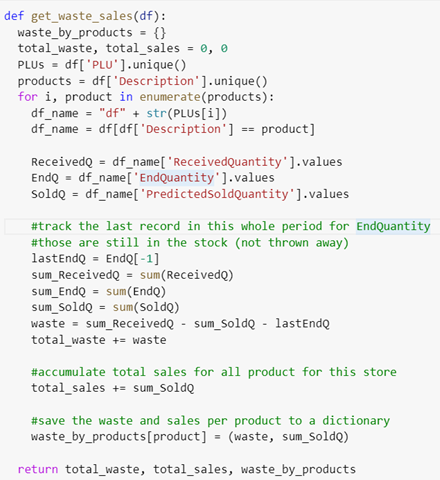
\includegraphics[width = 0.56\linewidth]{figures/algorithm.png}
\end{figure}

\subsection{Summary: Cost-Benefit Analysis among original data and all initiatives}
All the initiatives boost up enough sales to overwrite the wastes. Below table summarizes the overall increased percentage of profits comparing with the original dataset.


\begin{center}
\begin{tabular}{||c c c c||} 
 \hline
 Store ID & Original & Initiative 01 & Initiative 03\\ [0.7ex] 
 \hline\hline
 18 & baseline & 3 & 10\\ 
 \hline
 117 & baseline & 2 & 6 \\
 \hline
 332 & baseline & 4 & 15 \\ [1ex] 
 \hline
\end{tabular}
\end{center}

\subsubsection{Store 18} \\
Wastes (\$) = [3295, 3701, 4491]  \\
Sales (\$) = [43939, 45702, 49324] \\ 
Profits (\$) = [40644, 42001, 44833] \\
Original coffee store profit: \$40,644 \\
Initiative 1 profit: 42,001, profit increased 3\% \\
Initiative 3 profit: 44,833, profit increased 10\% \\

\begin{figure}[ht]
    \centering
    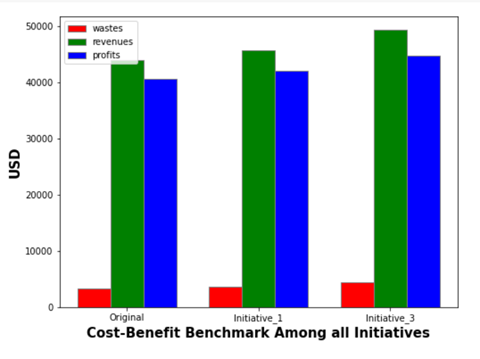
\includegraphics[width = 0.7\linewidth]{figures/section1.png}
\end{figure}

\newpage


\subsubsection{Store 117}  \\
Waste (\$) = [2454, 2812, 3591]  \\
Sales (\$) = [34451, 35289, 37476]  \\
Profits (\$) = [31997, 32477, 33885] \\
original coffee store profit: \$ 31997  \\
Initiative 1 profit: \$ 32477, profit increased 2\%  \\
Initiative 3 profit: \$ 33885, profit increased 6\%  \\

\begin{figure}[ht]
    \centering
    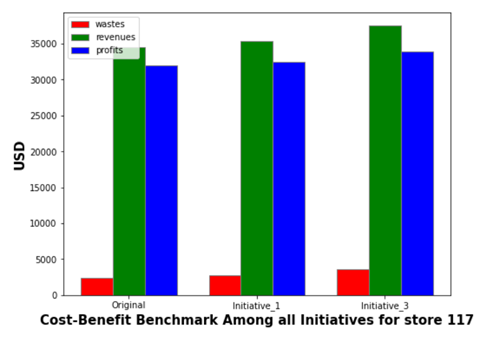
\includegraphics[width = 0.7\linewidth]{figures/section2.png}
\end{figure}

\subsubsection{Store 332}  \\
Wastes (\$) = [3203, 3597, 4453] \\
Sales (\$) = [83195, 87042, 96725] \\
Profits (\$) = [79992, 83445, 92272]\\
original coffee store profit: \$ 79, 992 \\
Initiative 1 profit: \$ 83,445, profits increase 4\%\\
Initiative 3 profit: \$ 92,272, profits increase 15\%\\

\begin{figure}[ht]
    \centering
    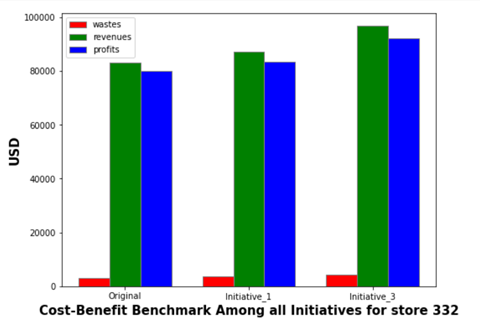
\includegraphics[width = 0.7\linewidth]{figures/section3.png}
\end{figure}

\subsection{Are the models conservative\?}
\textbf{Summary}
\begin{itemize}
    \item LSTM model is conservative to the different dataset. In general, the models are more conservative with the original dataset. With applying with initiatives (notice initiative 3 is more aggressive than initiative 1), we observe the model can predict to meet the higher demand of the market demands. 
    
\item Notice that there are outliers in the Sold Quantity (blue sharp up stream) that the model still misses. We believe those are triggers (similar to the initiatives we have applied, such as holidays, weather changes, weekday/weekends) that we can in further observe to apply more combinations to initiatives to catch the market needs.

\item We notice that a more risk-taking (risks regarding to potential wastes) results to more sales and higher profit. As a summary, the LSTM model is strong to adapt to different datasets to predict.

\end{itemize}

\textbf{Example: Store 18 of 820602 Everything Bagel }
The blue lines are the Received Quantity (either the original data or the adjusted data for each initiative); The read line are the predicted Sold Quantity for each dataset.

\begin{figure}[ht]
    \centering
    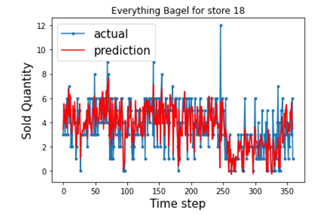
\includegraphics[width = 0.6\linewidth]{figures/section4.png}
    \caption{Original }
\end{figure}

\begin{figure}[ht]
    \centering
    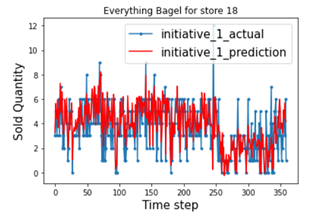
\includegraphics[width = 0.6\linewidth]{figures/section5.png}
    \caption{Initiative 1 (predicted sales based on the current initiative’s estimated Received Quantity) }
\end{figure}


\begin{figure}[ht]
    \centering
    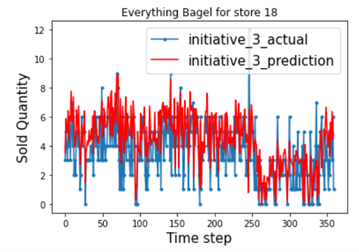
\includegraphics[width = 0.6\linewidth]{figures/section6.png}
    \caption{Initiative 3 (predicted sales based on the current initiative’s estimated Received Quantity) }
\end{figure}

\clearpage